\section{Topology Skeletons}
Even though many algorithms can be expressed by parallel maps, some problems require more sophisticated skeletons. The Eden library leverages this problem and already comes with more predefined skeletons, among them a \code{pipe}, a \code{ring} and a \code{torus} implementation \cite{eden_cefp, eden_skel_topology}. These seem like reasonable candidates to be ported to our arrow based parallel Haskell to prove that we can express such skeletons with Arrows as well.

\subsection{pipe}

The parallel pipe skeleton is semantically equivalent to folding over a list \code{[arr a a]} of arrows with \code{>>>}, but does this in parallel, meaning that the arrows don't have to reside on the same thread/machine. We implement this skeleton using the \code{ArrowLoop} typeclass which gives us the \code{loop :: arr (a, b) (c, b) -> arr a c} combinator which allows us to express loop like computations. For example this
\begin{lstlisting}[frame=htrbl]
loop (arr (\(a, b) -> (b, a:b)))
\end{lstlisting}
,which is the same as
\begin{lstlisting}[frame=htrbl]
loop (arr snd &&& arr (uncurry (:)))
\end{lstlisting}
defines an arrow that takes its input \code{a} and converts it into an infinite stream \code{[a]} of it. Using this to our advantage gives us a first draft of a pipe implementation by plugging in the parallel evaluation call \code{parEvalN conf fs} inside the second argument of \code{&&&} and then only picking the first element of the resulting list with \code{arr last}:
\begin{lstlisting}[frame=htrbl]
pipeSimple :: (ArrowLoop arr, ArrowParallel arr a a conf) =>
	conf -> [arr a a] -> arr a a
pipeSimple conf fs =
	loop (arr snd &&&
		(arr (uncurry (:) >>> lazy) >>> parEvalN conf fs)) >>>
	arr last
\end{lstlisting}
where \code{lazy} is defined as:
\begin{lstlisting}[frame=htrbl]
lazy :: (Arrow arr) => arr [a] [a]
lazy = arr (\ ~(x:xs) -> x : lazy xs)
\end{lstlisting}
Note that here the use of \code{lazy} is essential as without it programs using this definition would never halt. It is there so that the calculation of the input \code{[a]} halts before passing it into \code{parEvalN}.
\\\\
However, using this definition directly, will result in the master node becoming a potential bottleneck in distributed environments as described in chapter \ref{futures}. Therefore, a more sophisticated version that internally uses Futures is a good idea:
\begin{lstlisting}[frame=htrbl]
pipe :: (ArrowLoop arr, ArrowParallel arr (fut a) (fut a) conf,
	Future fut a) =>
	conf -> [arr a a] -> arr a a
pipe conf fs = unliftFut (pipeSimple conf (map liftFut fs))
\end{lstlisting}
Sometimes, this pipe definition can be a bit inconvenient, especially if we want to pipe arrows of mixed types together, i.e. \code{arr a b} and \code{arr b c}. By wrapping these two arrows inside a common type
\begin{lstlisting}[frame=htrbl]
pipe2 :: (ArrowLoop arr, ArrowChoice arr,
	ArrowParallel arr (fut (([a], [b]), [c])) (fut (([a], [b]), [c])) conf,
	Future fut (([a], [b]), [c])) =>
	conf -> arr a b -> arr b c -> arr a c
pipe2 conf f g = 
	(arr return &&& arr (const [])) &&& arr (const []) >>>
	pipe conf (replicate 2 (unify f g)) >>>
	arr snd >>>
	arr head
		where
			unify :: (ArrowChoice arr) =>
				arr a b -> arr b c -> arr (([a], [b]), [c]) (([a], [b]), [c])
			unify f g =
				(mapArr f *** mapArr g) *** arr (\_ -> []) >>>
				arr (\((a, b), c) -> ((c, a), b))
\end{lstlisting}
Note that extensive use of this combinator over \code{pipe} with a hand-written combination data-type will probably result in worse performance because of more communication overhead from the many calls to parEvalN. Nonetheless, we can define a parallel piping operator \code{|>>>|} which is semantically equivalent to \code{>>>} similar to the other parallel syntactic sugar from chapter \ref{syntacticSugar}:
\begin{lstlisting}[frame=htrbl]
(|>>>|) :: (ArrowLoop arr, ArrowChoice arr,
	ArrowParallel arr (fut (([a], [b]), [c])) (fut (([a], [b]), [c])) (),
	Future fut (([a], [b]), [c])) =>
	arr a b -> arr b c -> arr a c
(|>>>|) = pipe2 ()
\end{lstlisting}

\subsection{ring}
\begin{center}
	\includegraphics[scale=0.75]{images/ring}
\end{center}
Eden comes with a ring skeleton implementation that allows the computation of a function \code{[i] -> [o]} with a ring of nodes that communicate in a ring topology with each other. Its input is a node function \code{i -> r -> (o, r)} in which \code{r} serves as the intermediary output that gets send to the neighbour of each node. This data is sent over direct communication channels (remote data). The definition is as follows \cite{eden_skel_topology}:
\begin{lstlisting}[frame=htrbl]
ringSimple :: (Trans i, Trans o, Trans r) =>
   (i -> r -> (o,r))
   -> [i] -> [o]
ringSimple f is =  os
  where
    (os,ringOuts) = unzip (parMap (toRD $ uncurry f)
                                   (zip is $ lazy ringIns))
    ringIns = rightRotate ringOuts
\end{lstlisting}
with toRD (to make use of remote data)
\begin{lstlisting}[frame=htrbl]
toRD :: (Trans i, Trans o, Trans r) =>
        ((i,r) -> (o,r))
        -> ((i, RD r) -> (o, RD r))
toRD  f (i, ringIn)  = (o, release ringOut)
  where (o, ringOut) = f (i, fetch ringIn)
\end{lstlisting}
and rightRotate:
\begin{lstlisting}[frame=htrbl]
rightRotate    :: [a] -> [a]
rightRotate [] =  []
rightRotate xs =  last xs : init xs
\end{lstlisting}
We can rewrite its functionality easily with the use of \code{loop} as the definition of the node function, \code{arr (i, r) (o, r)}, after being transformed into an arrow, already fits quite neatly into the \code{loop}'s \code{arr (a, b) (c, b) -> arr a c}. In each iteration we start by rotating the intermediary input from the nodes \code{[fut r]} with \code{second (rightRotate >>> lazy)}. Similarly to the pipe, we have to feed the intermediary input into our \code{lazy} arrow here, or the evaluation would hang. The reasoning is explained by \cite{eden_cefp}:
\begin{quotation}
Note that the list of ring inputs ringIns is the same as the list of ring outputs ringOuts rotated by one element to the right using the auxiliary function rightRotate. Thus, the program would get stuck without the lazy pattern, because the ring input will only be produced after process creation and process creation will not occur without the first input.
\end{quotation}
Next, we zip the resulting \code{([i], [fut r])} to \code{[(i, fut r)]} with \code{arr (uncurry zip)} so we can feed that into a our input arrow \code{arr (i, r) (o, r)}, which we transform into \code{arr (i, fut r) (o, fut r)} before lifting it to \code{arr [(i, fut r)] [(o, fut r)]} to get a list \code{[(o, fut r)]}. Finally we unzip this list into \code{([o], [fut r])}. Plugging this arrow \code{arr ([i], [fut r]) ([o], fut r)} into the definition of \code{loop} from earlier gives us \code{arr [i] [o]}, our ring arrow.
\\\\
This gives us the following complete definition for the \code{ring} combinator:
\begin{lstlisting}[frame=htrbl]
ring :: (ArrowLoop arr, Future fut r,
	ArrowParallel arr (i, fut r) (o, fut r) conf) =>
    conf ->
    arr (i, r) (o, r) ->
    arr [i] [o]
ring conf f =
	loop (second (rightRotate >>> lazy) >>>
    arr (uncurry zip) >>>
    parMap conf (second get >>> f >>> second put) >>>
    arr unzip)
\end{lstlisting}
with \code{rightRotate}:
\begin{lstlisting}[frame=htrbl]
rightRotate :: (Arrow arr) => arr [a] [a]
rightRotate = arr $ \list -> case
	list of [] -> []
			xs -> last xs : init xs
\end{lstlisting}
and lazy:
\begin{lstlisting}[frame=htrbl]			
lazy :: (Arrow arr) => arr [a] [a]
lazy = arr (\ ~(x:xs) -> x : lazy xs
\end{lstlisting}
This combinator can, for example, be used to calculate the shortest paths in a graph using Warshall's algorithm. Further details on this can be found in \cite{eden_cefp}.
\subsection{torus}
\begin{center}
	\includegraphics[scale=0.75]{images/torus}
\end{center}
If we take the concept of a ring one dimension further, we get a torus. Every node sends ands receives data from horizontal and vertical neighbours in each communication round.
\\\\
With our parallel Arrows we implement a torus combinator yet again with the help of the \code{ArrowLoop} typeclass.
\\\\
Inside the loop we once again start by rotating the input, but this time not only in one direction, but in two. This means that the intermediary input from the neighbour nodes has to be stored in a tuple \code{([[fut a]], [[fut b]])} in the second argument (loop only allows for 2 arguments) of our input \code{([[c]], ([[fut a]], [[fut b]]))} and our rotation arrow becomes \code{second ((mapArr rightRotate >>> lazy) *** (arr rightRotate >>> lazy))} instead of the singular rotation in the ring as we rotate \code{[[fut a]]} horizontally and \code{[[fut b]]} vertically. We once again zip the inputs for the nodefunction with \code{arr (uncurry3 zipWith3 lazyzip3)} from \code{([[c]], ([[fut a]], [[fut b]]))} to \code{[[(c, fut a, fut b)]]}, which we then feed into our parallel execution.
\\\\
This, however, is more complicated than in the ring case as we have one more dimension of inputs to be transformed. We first have to \code{shuffle} all the inputs to then pass it into \code{parMap conf (ptorus f)} which yields us \code{[(d, fut a, fut b)]}. We can then unpack this shuffled list back to its original ordering by feeding this into the specific unshuffle arrow we created one step earlier with \code{arr length >>> arr unshuffle} with the use of \code{app} from the \code{ArrowApply} typeclass. Finally, we unpack this matrix \code{[[[(d, fut a, fut b)]]} with \code{arr (map unzip3) >>> arr unzip3 >>> threetotwo} to get  \code{([[d]], ([[fut a]], [[fut b]]))}.
\\\\
The complete definition of the \code{torus} combinator is:
\begin{lstlisting}[frame=htrbl]
torus :: (ArrowLoop arr, ArrowChoice arr, ArrowApply arr,
	ArrowParallel arr (c, fut a, fut b) (d, fut a, fut b) conf,
	Future fut a, Future fut b) =>
	conf -> arr (c, a, b) (d, a, b) -> arr [[c]] [[d]]
torus conf f =
	loop (second ((mapArr rightRotate >>> lazy) ***
		(arr rightRotate >>> lazy)) >>>
	arr (uncurry3 (zipWith3 lazyzip3)) >>>
	(arr length >>> arr unshuffle) &&&
		(shuffle >>> parMap conf (ptorus f)) >>>
	app >>>
	arr (map unzip3) >>> arr unzip3 >>> threetotwo)
\end{lstlisting}
with uncurry3,
\begin{lstlisting}[frame=htrbl]
uncurry3 :: (a -> b -> c -> d) -> (a, (b, c)) -> d
uncurry3 f (a, (b, c)) = f a b c
\end{lstlisting}
lazyzip3,
\begin{lstlisting}[frame=htrbl]
lazyzip3 :: [a] -> [b] -> [c] -> [(a, b, c)]
lazyzip3 as bs cs = zip3 as (lazy bs) (lazy cs)
\end{lstlisting}
ptorus,
\begin{lstlisting}[frame=htrbl]
ptorus :: (Arrow arr, Future fut a, Future fut b) =>
	arr (c, a, b) (d, a, b) ->
	arr (c, fut a, fut b) (d, fut a, fut b)
ptorus f =
	arr (\ ~(c, a, b) -> (c, get a, get b)) >>>
	f >>>
	arr (\ ~(d, a, b) -> (d, put a, put b))
\end{lstlisting}
and threetotwo.
\begin{lstlisting}[frame=htrbl]
threetotwo :: (Arrow arr) => arr (a, b, c) (a, (b, c))
threetotwo = arr $ \ ~(a, b, c) -> (a, (b, c))
\end{lstlisting}
As an example of using this skeleton \cite{eden_cefp} gave the matrix multiplication using the gentlemans algorithm. Adapting this nodefunction to our arrow API gives us:
\begin{lstlisting}[frame=htrbl]
nodefunction :: Int ->
	((Matrix, Matrix), [Matrix], [Matrix]) ->
	([Matrix], [Matrix], [Matrix])
nodefunction n ((bA, bB), rows, cols) =
	([bSum], bA:nextAs , bB:nextBs)
		where bSum =
			foldl' matAdd (matMult bA bB) (zipWith matMult nextAs nextBs)
			nextAs = take (n-1) rows
			nextBs = take (n-1) cols
\end{lstlisting}
If we compare the trace from a call using our arrow definition of the torus (fig. \ref{fig:torus_parrows_trace}) with the Eden version (fig. \ref{fig:torus_eden_trace}) we can see that the behaviour of the arrow version is comparable.
\begin{figure}[ht]
	\centering
	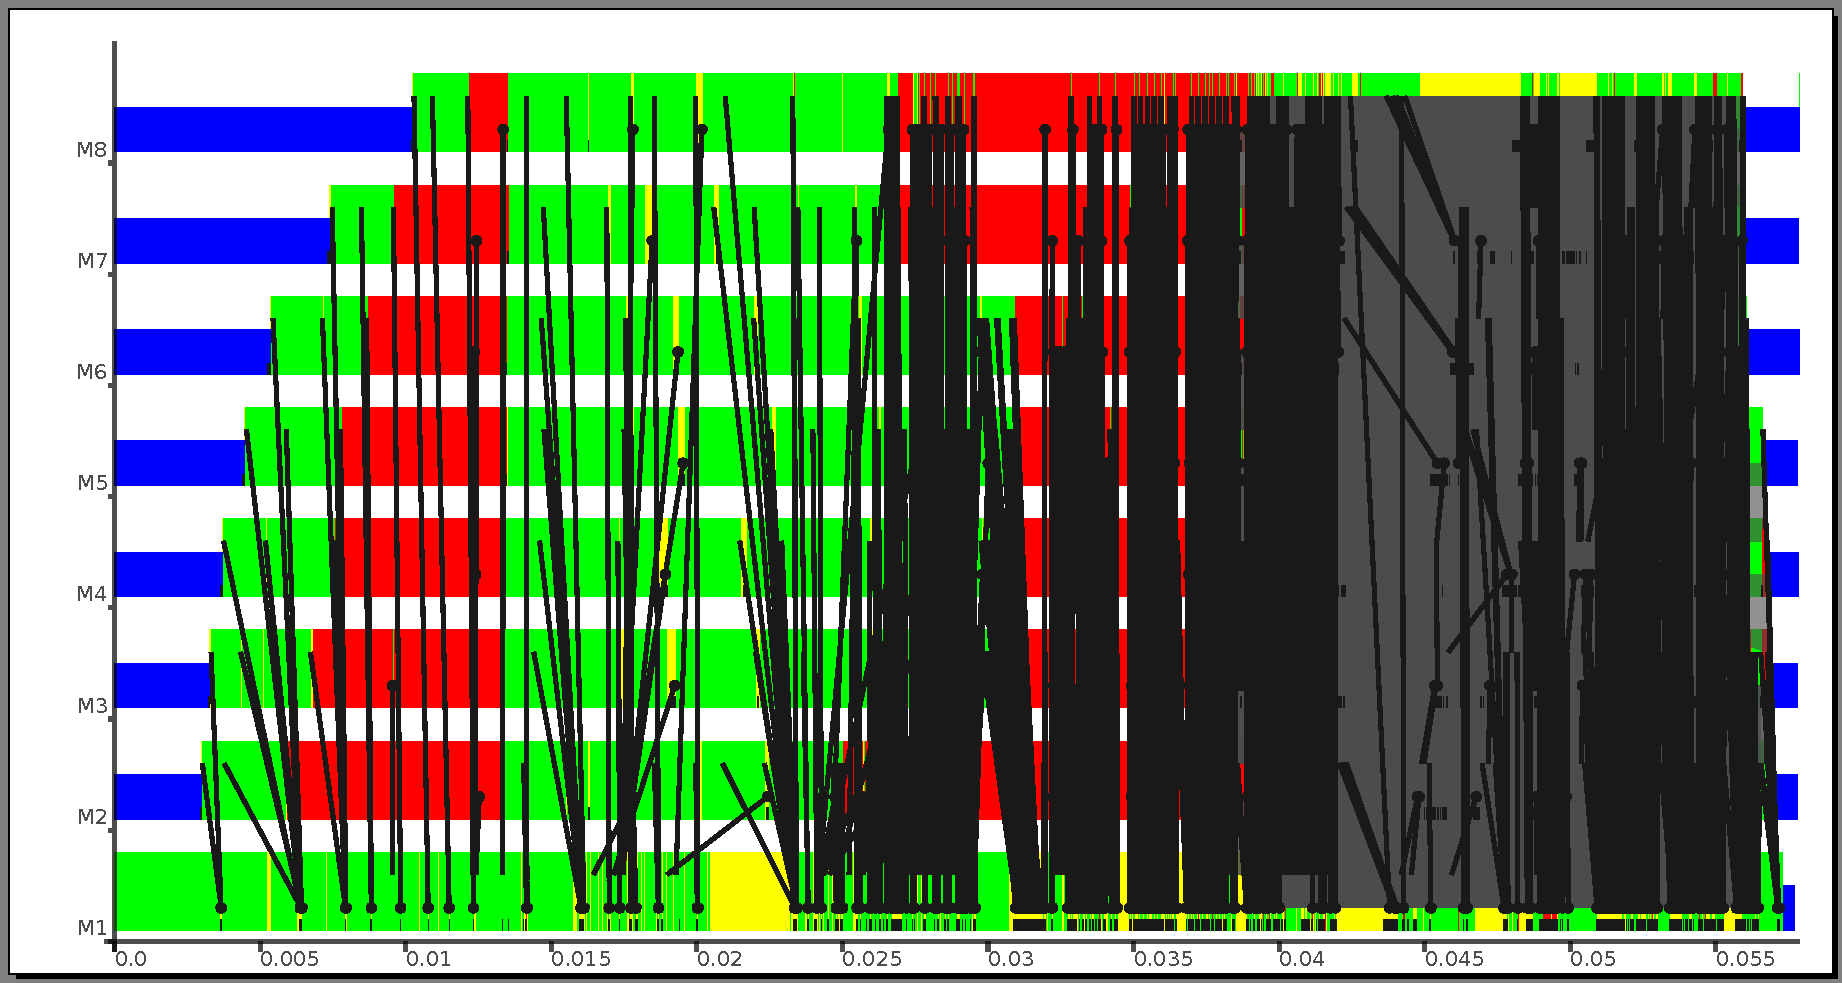
\includegraphics[width=0.9\textwidth]{images/torus_matrix_parrows_scale}
	\caption[Matrix Multiplication with a torus (Parrows)]{Matrix Multiplication with a torus (Parrows)}
	\label{fig:torus_parrows_trace}
\end{figure}

\begin{figure}[ht]
	\centering
	\includegraphics[width=0.9\textwidth]{images/torus_matrix_eden_scale}
	\caption[Matrix Multiplication with a torus (Eden)]{Matrix Multiplication with a torus (Eden)}
	\label{fig:torus_eden_trace}
\end{figure}

%\begin{figure}[ht]
%	\centering
	\framebox{
		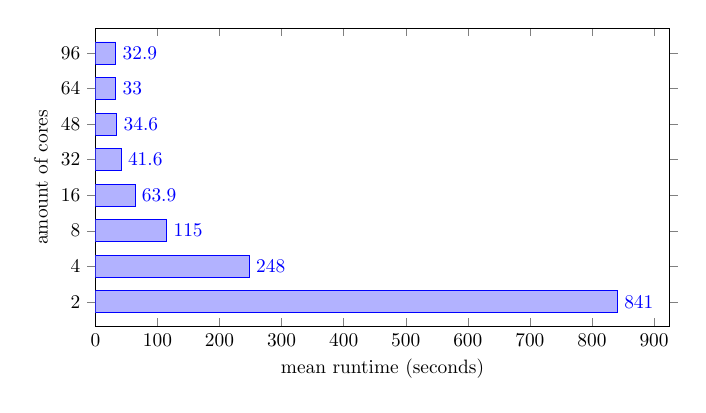
\begin{tikzpicture}[thick, scale=0.7]
		\begin{axis}[
			xbar, xmin=0,
			bar width=0.4cm,
			width=12cm, height=7cm, enlarge y limits=0.1,
			ylabel={amount of cores},
			xlabel={mean runtime (seconds)},
			symbolic y coords={2, 4, 8, 16, 32, 48, 64, 96},
			ytick=data,
			nodes near coords, nodes near coords align={horizontal},
			]
			\addplot coordinates {(841,2) (248,4) (115,8) (63.9,16) (41.6,32) (34.6,48) (33.0,64) (32.9,96)};
		\end{axis}
		\end{tikzpicture}
	}
%	\caption[Parallel Matrix Multiplication using Eden (two 1024x1024 matrices)]
%\end{figure}

\framebox{
	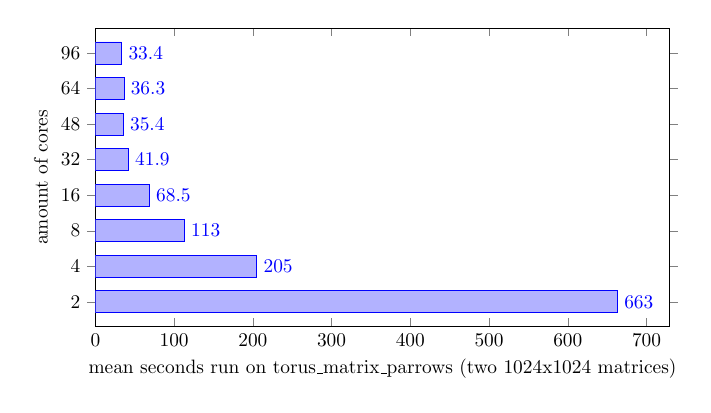
\begin{tikzpicture}[thick, scale=0.7]
	\begin{axis}[
	xbar, xmin=0,
	bar width=0.4cm,
	width=12cm, height=7cm, enlarge y limits=0.1,
	ylabel={amount of cores},
	xlabel={mean seconds run on torus\_matrix\_parrows (two 1024x1024 matrices)},
	symbolic y coords={2, 4, 8, 16, 32, 48, 64, 96},
	ytick=data,
	nodes near coords, nodes near coords align={horizontal},
	]
	\addplot coordinates {(663,2) (205,4) (113,8) (68.5,16) (41.9,32) (35.4,48) (36.3,64) (33.4,96)};
	\end{axis}
	\end{tikzpicture}
}
